\section{Non functional requirements}
\label{section:technicalReq}
The requirements specified in this section present us the technical/non-functional aspects of the Archive service. A tabular description 
(Table \ref{table: Technical Requirements}) is presented below.
The detailed description depicts the benchmarks of how the system should be designed to meet the needs for a better sustainable prototype.
The result from this work delivered must comply with the following technical requirements.

    \begin{longtable}{|p{3cm}|p{12cm}|}
            \hline
                \textbf{Requirement}  & \textbf{Description}\\
            \hline
                 Build and deployment & 
                 The service should be deployable in the MARS kubernetus \cite{kubernetes} cluster using the Gitlab pipeline as seen in Figure \ref{fig:CIbuild}
                 which is valid at the time of writing this Thesis. In addition,
                 the build stages for the pipeline also has to be written. \\
            \hline
                Docker containerizing.
                & Choose a suitable Docker container \cite[p.~7 - 8]{Torre2017} for the service. This depends on the type of programming language which 
                the service is being
                written in (e.g. dotnet core, python, java, go).\\
            \hline
                 Scalability & Provide further extensibility option using object orientation so that the service can be scalable.\\
            \hline
                 Robustness & The system should be tested against multiple cases to ensure correct functionality of the service using unit tests and
                 integration tests.\\    
            \hline
                 Performance & The duration of the archive and retrieve process should be measurable. So that a close watch on the performance of the system is 
                 possible. \\    
            \hline
                 Usability & The system should be integrated in the MARS UI so that it is easily usable by all end users.\\    
            \hline
                 Connection to Synology & The Archive service should be able to make a connection to the Synology drive and store desired data successfully.\\ 
            \hline
                 Make a Swagger API interface & The Archive service should have a Swagger \cite{swagger} interface available so that other 
                 developers can use the service with ease.\\         
            \hline
                Follow Microservice patterns & The service should follow data sovereignty pattern for Microservices mentioned in 
                (Subsection \ref{subsection:dataSovereignty}).\\ 
            \hline
                Responsiveness & The API should give some kind of feedback to the user never the less if request cannot be made an 
                error message should be returned instead of no result. \\      
            \hline
        \caption{Technical requirements for the Archive service}
        \label{table: Technical Requirements}     
    \end{longtable} 
  
    \begin{figure}[H]
        \centering 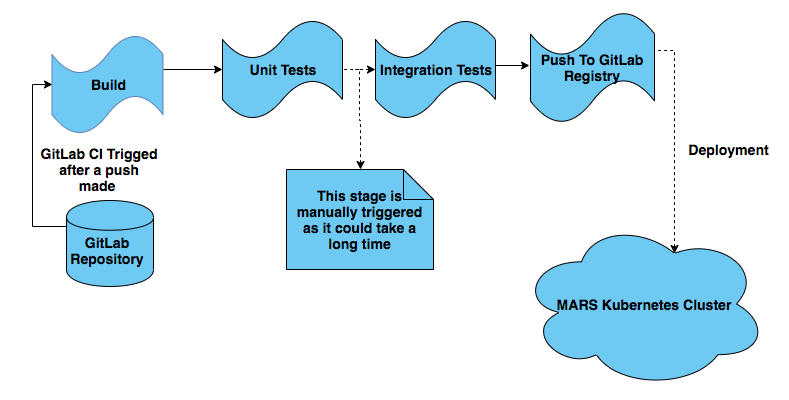
\includegraphics[scale=0.5]{grafiken/CIbuild.png}
        \caption{MARS Continuous Integration Pipeline build}
        \label{fig:CIbuild}
    \end{figure}

    Figure \ref{fig:CIbuild} presents the Continuous Integration system which is being followed at the time of writing this thesis by the MARS developer community.
    The CI\footnote{CI: Continuous Integration} pipeline would be triggered as soon as a new commit is being pushed to the remote 
    GitLab\footnote{https://about.gitlab.com} repository. This would then build the docker image of the service with the new changes. The next step would be to
    run the unit tests written for the service, which is a mandatory step. Lastly, if the pipeline passes, the docker image will be pushed
    to the GitLab registry\footnote{https://about.gitlab.com/2016/05/23/gitlab-container-registry/}. If this is successful then the image can be used in one of 
    the MARS kubernetes cluster i.e. MARS beta, MARS production environments. In addition,
    it can be seen that the integration tests are configured to be an optional test because the integration tests could consume considerably more time and may hinder
    important updates. For this reason, the integration tests are ran manually in the pipeline.